% 2008 年广东卷文科第 18 题：四棱锥 P-ABCD，底面 ABCD 是半径为 R 的圆的内接四边形，
%   BD 是圆的直径，∠ABD=60°，∠BDC=45°，△ADP∽△BAD。
% 来源 PDF：gaokaomath-src/普通高考/2008/2008广东文.pdf
% SHA-256：1adedadb12b82b7b4d04721908bd686e747021593ec91da14b0e4e979929373c
% 原页：2008广东文.pdf 第 2 页（A3 三栏）第 1 栏，书页码 448。
% 重绘依据：底面圆画成椭圆，前半个椭圆（A→B→C→D）为实线、后半个为虚线；
%   A、B、C、D 均在椭圆上且 B、D 关于中心对称（BD 为直径），AD、BD 被遮挡用虚线。
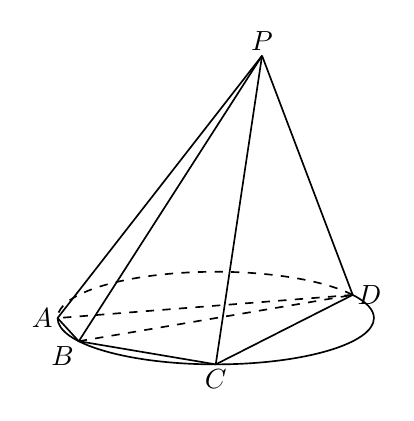
\begin{tikzpicture}[scale=0.98, semithick, every node/.style={inner sep=1.5pt}]
  % 底面椭圆：中心 (2.70,1.15)，半长轴 2.05、半短轴 0.60
  \coordinate (O) at (2.70,1.15);
  \coordinate (A) at (0.65,1.15);
  \coordinate (B) at (0.925,0.85);
  \coordinate (C) at (2.70,0.55);
  \coordinate (D) at (4.475,1.45);
  \coordinate (P) at (3.30,4.55);

  % 底面椭圆：后半（D→上→A）虚线，前半（A→下→D）实线
  \draw[dashed] (D) arc[start angle=30, end angle=180, x radius=2.05, y radius=0.60];
  \draw (A) arc[start angle=180, end angle=390, x radius=2.05, y radius=0.60];

  % 底面四边形的边
  \draw (A) -- (B) -- (C) -- (D);
  \draw[dashed] (D) -- (A);
  \draw[dashed] (B) -- (D);

  % 侧棱
  \draw (P) -- (A);
  \draw (P) -- (B);
  \draw (P) -- (C);
  \draw (P) -- (D);

  \node[above] at (P) {$P$};
  \node[left] at (A) {$A$};
  \node[below left] at (B) {$B$};
  \node[below] at (C) {$C$};
  \node[right] at (D) {$D$};
\end{tikzpicture}
